\chapter{Dostupné platformy}

\label{lego-soft-available-platforms}


Pro \legoEV{} existuje mnoho vývojových platforem. 
Většinou se jedná o~specificky navržené programovací API ve~spojení s~vývojovým prostředím. 
Tyto platformy často fungují ve~spolupráci s~oficiálním systémem v~\EVthree{}, ale jsou i~platformy s~vlastním operačním systémem. 
V~tomto textu bude popsán jen výběr těch nejzajímavějších. % platforem. 

\section{Originální prostředí od \lego}

V~rámci této podkapitoly je rozebírán samotný operační systém na \EVthree{} a~také vývojové prostředí, určené pro tvorbu a~ladění programů. 
\lego{} si pro \EVthree{} vytvořilo vlastní operační systém, postavený na linuxovém jádru \cite{legoMindstormsEV3_fw-dev-kit}. 
Uvnitř systému běží virtuální stroj, který zpracovává byte-code uživatelské aplikace. 
Byte-code je vytvořen ve~vývojovém prostředí na PC a~pak je do \brick{\it u} odeslán po USB kabelu, Bluetooth nebo WiFi.

Celý systém s~vývojářskými nástroji a~dokumentací je volně k~dispozici na~webu \lego{}~\cite{legoMindstorms_download}. Jelikož~\lego{} uvolnilo zdrojové kódy, mohly vzniknout alternativní systémy pro~\EVthree{} jako~\evThreeDev{} (kapitola~\ref{lego-ev3dev}) nebo \evRT{} (kapitola~\ref{lego-EV3RT}). 

\subsection{\legoSW{}}
\label{lego-soft-orig-problems}


\begin{figure}[h]
	\centering
	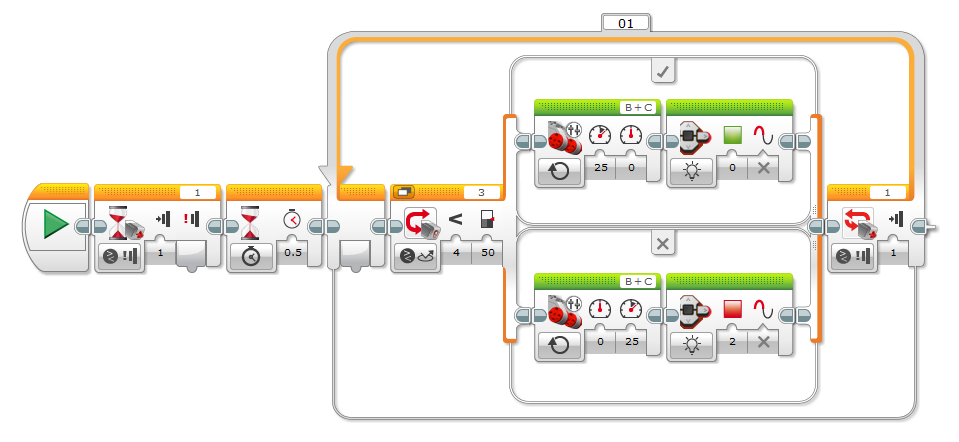
\includegraphics[width=0.99\textwidth]{images/lego-soft_robotut_switch-touch+motors+leds.png}
	\caption{Ukázka programovacích bloků v~\legoSW}
	\label{fig:lego-soft_example-blocks}
\end{figure}

\legoSW{} je~vývojářský program, který je k~\EVthree{} dostupný zdarma. 
Tento  software vytvořilo \lego{} ve~spolupráci s~firmou \NI{}. 
Je~tudíž postavený na~vývojovém prostředí \labview{}. 
\lego{} s~\NI{} již~spolupracovalo na předešlých vývojových prostředích. 
Program se~snaží působit jako profesionální vývojové a~laboratorní studio, což se~mu celkem daří.
Nabízí celou řadu funkcí od modulu pro programování přes tvorbu různých experimentů až~po přípravy interaktivních návodů a~průvodců programováním v~tomto prostředí.

V~režimu tvorby programu jsou hlavními stavebními kameny \EVblocks, které se ve~formě diagramů skládají do podoby výsledného programu (obrázek \ref{fig:lego-soft_example-blocks}).
Bloky jsou rozděleny do~několika skupin (akční, tok programu, senzory, datové operace, pokročilé a~vlastní), které se liší svojí barvou a~použitím. 
Pomocí těchto bloků lze řídit tok programu (podmínky, cykly, čekání a~vlákna), pracovat s~proměnnými, obsluhovat motory či senzory, provádět matematické operace anebo i~využívat vlastní bloky.

\begin{figure}[h]
	\centering
	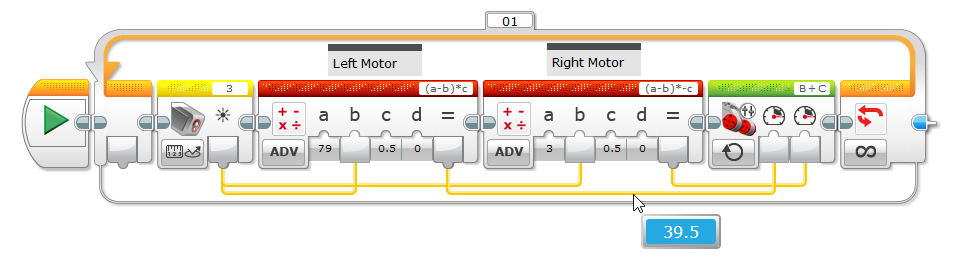
\includegraphics[width=\textwidth]{images/lego-soft_live-debugging_line-advance.png}
	\caption{Ukázka debuggování za běhu programu}
	\label{fig:lego-soft_live-debugging_line-advance}
\end{figure}

Vše je pěkně graficky zpracováno a~působí jako jednotný celek. 
Při běhu programu lze~sledovat jeho tok (kde v~diagramu se program nachází) nebo si třeba zobrazit aktuální stav (hodnotu proměnné, výsledek matematické operace, vstupní data ze~senzoru, \dots). 
Ukázku debuggování si~lze prohlédnout na obrázku \ref{fig:lego-soft_live-debugging_line-advance}, kde je vidět hodnota 39.5, odpovídající výsledku výpočtu výkonu pro levý motor v~závislosti na~naměřené hodnotě od barevného senzoru.
Zároveň je podle šrafování vrchní lišty bloků vidět, že~program aktuálně probíhá v~daném cyklu.

Pro práci s~\brick{\it em} je k~dispozici modul {\it Správa hardwaru}, kde si lze zjistit informace jako jméno, stav baterie, verze firmwaru nebo obsazenost paměti. 
Umožňuje také jednoduše nahrávat, spouštět a~ukončovat programy. 

Nalezneme zde i~správu připojení, v~rámci které lze vyhledávat a~připojovat se k~dostupným \brick{\it ům}. 
K~dispozici jsou tři druhy připojení: USB kabel, Bluetooth a~WiFi. Bluetooth je již integrován, ale pro použití WiFi je potřeba připojit WiFi modul.

\begin{figure}[h]
	\begin{minipage}[b]{.48\textwidth}
		\centering
		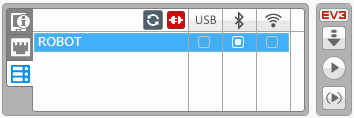
\includegraphics[width=\textwidth]{images/lego-soft_brick-manager_connected.png}
		\caption{Správa připojení k~\brick{\it u}}
		\label{fig:lego-soft_brick-manager-connected}
	\end{minipage}
	\hfill
	\begin{minipage}[b]{.48\textwidth}
		\centering
		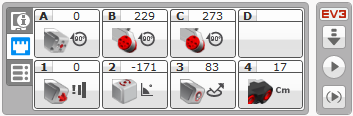
\includegraphics[width=\textwidth]{images/lego-soft_brick_port-view.png}
		\caption{Informační panel s~porty}
		\label{fig:lego-soft_brick_port-view}
	\end{minipage}
\end{figure}

Nejzajímavějším panelem je správce portů (obrázek~\ref{fig:lego-soft_brick_port-view}). 
Zobrazuje, na jakém portu je připojen který senzor nebo motor. 
Uživatel může vidět také aktuální hodnoty komponentů a~přepínat jejich režimy.    
Například u~barevného senzoru si~může vybrat, zda se bude zobrazovat barva, nebo odrazivost povrchu. U~motorů lze naopak nastavit, jestli má být ujetá vzdálenost zobrazování v~otáčkách, nebo ve~stupních. 
Tento panel považuji ze jednu z~nejpodstatnějších funkcí celého programu, jelikož dává uživateli dobrý přehled o~aktuálním stavu hardwaru. 
Jednoduše lze tak ladit konstanty v~programech (rozhodovací úroveň pro barevný senzor při detekci čáry, počet otáček motoru potřebných k~dojetí na~požadovanou pozici nebo vzdálenost od~překážky naměřenou ultrazvukem). 

V~následujících odrážkách je shrnut výčet nevýhod a~nedostatků originálního LEGO prostředí. 
Za nejdůležitější bod bych považoval nepřehlednost rozsáhlejších programů. % a nemožnost ladění a úpravy uživatelských bloků. 


To je pravděpodobně hlavní důvod, proč uživatelé \legoM{} vyhledávají alternativní prostředí. 
Ukázku rozsáhlejších programů je možné vidět na~obrázcích \ref{fig:lego-soft_legolib_converge_array}~a~\ref{fig:lego-soft_legolib_match_array_length}.\\

Nevýhody \legoSW:

\renewcommand{\labelitemi}{$-$} % nastavení pomlček místo plných koleček
\begin{itemize}[noitemsep]\itemsep2pt
	\item náročný na hardware počítače
	\item ve větších programech je obtížné se zorientovat anebo najít chybu
	\item nelze editovat proměnné ani rozhraní uživatelských bloků (jejich parametry)
	\item debuggovací režim nefunguje uvnitř uživatelských bloků
	\item při rozsáhlejších programech přestává prostředí fungovat (zamrzá a~padá)
	\item není dostupný na Linuxu a~není open-source
\end{itemize}

Nevýhody operačního systému v~\brick{\it u}:
\begin{itemize}[noitemsep]\itemsep2pt
	\item dlouhé zapínání a~vypínání
	\item značně pomalé zpracovávání některých operací (\dots) % TODO: dopsat operace
	\item nepracuje v~real-time režimu a~časování jednotlivých operací tedy není garantováno
	\item podpora jen jednoho typu WiFi modulu
\end{itemize}
\renewcommand{\labelitemi}{$\bullet$} % vrácení zpět plných koleček

\begin{figure}[h]
	\centering
	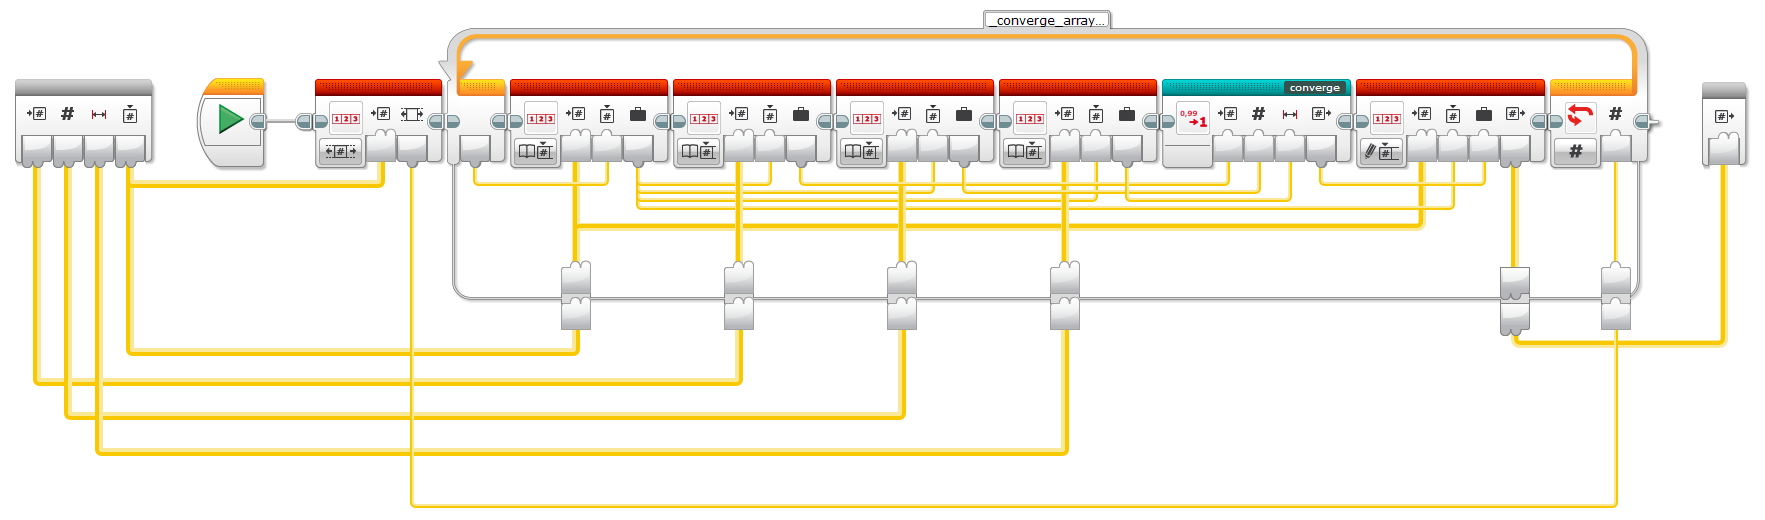
\includegraphics[width=\textwidth]{images/lego-soft_legolib_converge_array.png}
	\caption[Ukázka nepřehlednosti rozsáhlejších programů]{Ukázka nepřehlednosti rozsáhlejších programů - žluté dráhy značí předávání vstupních a~výstupních parametrů mezi jednotlivými bloky - velmi špatně se zjišťuje a~kontroluje správnost zapojení žlutých drah.}
	\label{fig:lego-soft_legolib_converge_array}
\end{figure}
 
\legoSW{} lze nainstalovat na operační systémy Windows a~Mac. K~dispozici jsou i~aplikace s~omezenými možnostmi programování pro tablety na platformě Android a~iPady.


\section{ev3dev}
\label{lego-ev3dev}

Platforma \evThreeDev{}~\cite{legoMindstormsEV3_ev3dev} je pravděpodobně nejrozšířenější a~nejrozsáhlejší alternativa k~originálnímu \lego{} prostředí.
Jedná se o~systém, drivery a~různé wrappery pro jednotlivé programovací jazyky. 
Samotný systém je založený na~linuxové distribuci Debian, který má v~sobě naportovány originální \lego{} drivery pro \EVbrick{} a~veškeré periferie.

Jelikož je \evThreeDev{} postaven na standardní linuxové distribuci, lze používat velkou škálu programovacích jazyků. 
K~dispozici jsou nízkoúrovňové jazyky C~a~C++. 
Připraveny jsou i~knihovny a~wrappery pro Python, JavaScrip, Go~\cite{legoMindstormsEV3_ev3dev-prog-lang}. 
Každý si zde může vybrat podle svých zkušeností nebo preferencí a~v~případě chuti naimplementovat i~podporu pro další jazyky. 
Aktuálně jsou stále rozpracovány implementace pro Java, Lua, Ruby,~\dots{}.

Pro práci se systémem je k~dispozici SSH~připojení, případně lze využít terminál dostupný na~úvodní obrazovce a~přes USB port si~připojit externí klávesnici. 
Tento způsob ale z~důvodu velikosti displeje na \brick{\it u} není moc komfortní. 
Systém \evThreeDev{}, na~rozdíl od~originálního \lego{} prostředí, má lepší podporu ovladačů pro WiFi a~funguje prakticky s~jakýmkoliv USB modulem. 
Systém umožňuje nastavení automatického připojování na konkrétní WiFi. Pak se již lze k~\brick{\it u} připojovat bezdrátově.
K~připojení je možné případně použít i~USB Ethernet modul.
 
Co se týče podpory \lego{} motorů a~senzorů, \evThreeDev{} zvládá obsluhovat všechny typy určené pro EV3, NXT a~některá zařízení z~WeDo~\cite{legoMindstormsEV3_ev3dev-support-motors}~\cite{legoMindstormsEV3_ev3dev-support-sensors}.
Je implementována i~široká podpora alternativních výrobců jako mindsensors.com nebo HiTechnic~\cite{baichtal2016hacking}. 
Mindsensors.com na svých webových stránkách u~některých modelů zmiňují i~podporu \evThreeDev{}~\cite{lego_mindsensor_gyro}.  

Pro zajímavost lze dodat, že tento systém podporuje i~alternativní \brick{\it y} postavené na jednodeskových počítačích Raspberry~Pi nebo BeagleBone. Příkladem komerčně prodávaných \brick{\it ů} jsou BrickPi od~Dexter Industries~\cite{lego_dexterindustries_brickpi} a~PiStorms od mindsensors.com~\cite{lego_mindsensor_pistorms}.
Obě tyto alternativy jsou postaveny na Raspberry~Pi a~umožňují připojit stejný počet standardních \lego{} motorů a~senzorů jako EV3.
Jejich hlavní výhodou je přítomnost výrazně výkonnějšího procesoru v~Raspberry~Pi. Na klasickém \brick{\it u} je totiž \evThreeDev{} dosti pomalý. 
Například samotný start systému trvá přes 60~sekund~\cite{legoMindstormsEV3_ev3dev_video-system-boot}. 
Otevření SSH spojení přes WiFi, nahrání binárního souboru do \brick{\it u} a~následné spuštění zabere až 40~sekund. 
K~tomuto zdlouhavému procesu bohužel dochází při každé změně programu. 
Díky použití Raspberry~Pi je také možné jednoduše připojit například kameru anebo přímo na GPIO piny přidat vlastní senzory (měření teploty, tlaku, vlhkosti, hodiny reálného času,~\dots).  
Mezi nevýhody můžeme počítat nemožnost účasti s~těmito alternativními \brick{\it y} soutěží, které jsou striktně omezeny na použití jen \lego{} komponent (v~České republice: \fll{}, Robosoutěž ČVUT, Robotiáda).

Avšak i~tento systém trápí podobné problémy jako originální \lego{} prostředí. 
Hlavním nedostatkem je, že~Linux nemá standardně real-time kernel. 
% Linux -> scheduler -> spravedlivý -> negarantuje čas, ale optimální využití procesoru
% real-time -> není spravedlivý ale umožňuje přesné časování jednotlivých tasku a přesné cyklické spouštění tasku -> nedochází k optimálnímu využití procesoru
Není tak garantováno přesné přidělování výpočetního času pro uživatelské programy, což je velký problém pro běh různých regulačních smyček, které potřebují konstantní dobu mezi jednotlivými průběhy (například stabilizace samobalancujícího robota). 
V~\evThreeDev{} dle měření dochází až k~20~ms prodlevám, kdy si kernel zabere výpočetní čas a~uživatelská aplikace se nedostane k~vykonávání programu~\cite{legoMindstormsEV3_ev3dev-issue_constant-loop-time}. 
Jedno z~řešení je výrazně zpomalit regulační smyčku, ale ani to negarantuje, že se program dostane k~vykonávání v~požadovaný čas.
V~rámci \evThreeDev{} proběhl pokus o~zakomponování real-time kernelu do separátní vývojové větve.~\cite{legoMindstormsEV3_ev3dev-rt-kernel-start}. 
Jelikož se ale tato větev potýkala s~problémy ovladačů motorů, byl její vývoj ukončen~\cite{legoMindstormsEV3_ev3dev-rt-kernel-end}.  
% TODO: scheduler v EV3 -  https://github.com/ev3dev/ev3dev/issues/324
%Určité výtky lze mít i~vůči implementaci driverů pro motory, kde se většina nastavování provádí přes textové řetězce (viz~obrázek~\ref{src:ev3dev-lang-cpp_drive-test}). 
%Určitě se nejedná o nejrychlejší řešení.


\begin{figure}[H] 
	\begin{minted}[xleftmargin=1.5em,linenos=true]{cpp}
if(motor.speed_regulation_enabled() == "off")
    motor.set_speed_regulation_enabled("on");
motor.set_speed_sp(speed);
motor.run_forever();
	\end{minted}
	\caption{Ukázka nastavení rychlosti motoru v~implementaci C++ na \evThreeDev}
	\label{src:ev3dev-lang-cpp_drive-test}
\end{figure}

Co považuji za~další problém, je roztříštěnost této platformy a~náročnost pro méně zkušené uživatele. 
Jednotlivé implementace programovacích jazyků mají různorodou kvalitu dokumentace a~většinou relativně složité rozhraní. 
Na obrázku~\ref{src:ev3dev-lang-cpp_drive-test} je ukázka kódu pro nastavení rychlosti jednoho motoru v~C++~na~\evThreeDev{}. 
Pro další inspiraci je možné se podívat na~demo příklady k~tomuto API~\cite{legoMindstormsEV3_ev3dev-lang-cpp_drive-test}.
Bohužel pro člověka, který doposud programoval pouze přes \lego{} prostředí, je podle mě toto rozhraní velmi složité.

%Jelikož mám na~\evThreeDev{} největší zkušenosti s C++~API, tak bych chtěl poukázat na nedostatky v tomto API. 
%Zároveň by u~C++ nemělo docházet k~degradaci výkonu, což může nastávat u interpretovaných jazyků jako Python nebo JavaScript. 
Příklad v~C++~API jsem vybral z~důvodu svých předešlých zkušenosti s~tímto rozhraním a~předpokladu, že by u~C++ nemělo docházet k~degradaci výkonu, což by mohlo nastávat u~interpretovaných programovacích jazyků jako Python nebo JavaScript.

Ze~svých dlouhodobých zkušeností se~začátečníky mám dobrou představu, jakých chyb se nejčastěji dopouští a~co jim dělá největší problém.
Proto jsem se v~rámci testování \evThreeDev{} podílel i~na tvorbě knihovny~\cite{legoMindstormsEV3_ev3dev_RB-ev3dev-cpp-lib}, která byla vyvíjena se záměrem co nejvíce usnadnit uživateli programování robotů v~\evThreeDev{}. 
Přestože tato knihovna mnohé neduhy programování na tomto systému odstraňuje, stále tu přetrvává celá řada problémů souvisejících s~použitím linuxového systému (viz popis v~úvodu této kapitoly).


Při zkoumání API pro Python~\cite{legoMindstormsEV3_ev3dev-lang-python} jsem došel k~podobnému závěru. 
Je pravda, že k~němu lze najít rozsáhlejší dokumentaci~\cite{legoMindstormsEV3_ev3dev-lang-python-docs}. 
I~tak není dle mého názoru pro programátora~- začátečníka, který přechází z~\lego{}  softwaru, toto API dostatečně jednoduché a~intuitivní.


\section{ROS}

S~\legoEV{} je možné používat i~ROS (Robot Operating System)~\cite{legoProgramingPlatform_ROS}. 

ROS je platforma určená přímo pro robotiku a~roboty. 
Jde o~systém, který v~sobě integruje nástroje pro komunikaci, loggování, zpracování obrazu, navigaci, simulace nebo ovládání zařízení. 
Uživateli značně usnadňuje obsluhu vlastního robota, protože má předpřipraveno již mnoho nástrojů.

Na samotném EV3 kvůli nedostatečnému výkonu \brick{\it u}  kompletní ROS neběží.
Pro EV3 ale existuje utilita do systému \evThreeDev{}, přes kterou lze pomocí příkazů komunikovat s~ROSem běžícím na standardním PC. 
Tím lze získávat data ze senzorů a~posílat zpět instrukce pro motory. 
Komunikace mezi PC a~\EVbrick{\it em} může probíhat po WiFi nebo Ethernetu.
Veškerá logika jako plánování trasy, herní strategie, případně zpracování dat je prováděna v~rámci klasického~PC.
Hlavními důvody pro použití ROSu na EV3 je široká paleta balíčků, které řeší například práci s~různými senzory jako kamera, Kinect, lidar, ale i~ovládacích zařízení typu joystick či gamepad. 
Zároveň je v~ROSu integrována transformace souřadnic, plánování trasy, herní strategie nebo i~simulátor s~fyzikálním enginem.


Při využívání ROSu společně se stavebnicí \lego{} je ovšem problematická nutnost mít k~\brick{\it u} připojené klasické PC. 
Jak bylo již uvedeno v~kapitole~\ref{lego-ev3dev}, mnoho soutěží pro \legoM{} vyžaduje striktní použití jen \lego{} komponent, a~to běžné PC není. 
Zároveň i~soutěže, které nemají tuto podmínku, například Robotický den v~Praze nebo Istrobot v~Bratislavě, zakazují spojení s~jakýmkoliv externím zařízením.
Tím pádem je nutné, aby na sobě \lego{} robot vozil klasické PC, což může značně zvýšit hmotnost a~náročnost konstrukce. 
V~dnešní době by to ovšem již neměl být takový problém (např. lze použít Raspberry~Pi anebo zařízení založené na~Intel Atom).

\section{Balíček od MathWorks}
\label{lego-alternative-soft_mathworks}

MathWorks pro \legoM{} připravil doplňky do svých programů Matlab a~Simulink. 
Cílem těchto doplňků je umožnit uživateli ovládat a~programovat \legoM{} ve standardním MathWorks prostředí. 
V~rámci balíčků je podporováno \legoNXT~\cite{legoProgramingPlatform_MathWork-NXT} i~EV3~\cite{legoProgramingPlatform_MathWork-EV3}.
Uživatel může ovládat \brick{} pomocí příkazů z~Matlabu anebo lze program vytvořit formou diagramů v~Simulinku (podobně jako v~oficiálním \lego{} prostředí). 
Příklad programu pro sledování čáry lze vidět na obrázku~\ref{fig:mathworks-simulink_line-tracking-model}.
Programy v~Simulinku vypadají srozumitelně a~přehledně, ale vzhledem k~povaze samotného prostředí (laboratorní až~vědecký simulační nástroj) není jeho ovládání a~tvorba aplikací jednoduchá a~pro nováčka občas až odrazující. 

\begin{figure}[h]
	\centering
	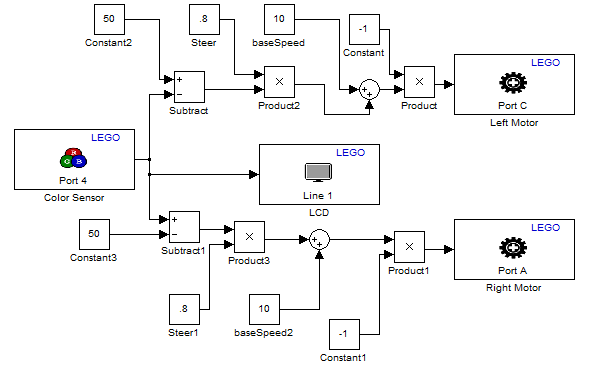
\includegraphics[width=330px]{images/mathworks-simulink_line-tracking-model.png}
	\caption[Program na sledování čáry v~prostředí Simulink]{Program na sledování čáry v~prostředí Simulink\protect\footnotemark}
	\label{fig:mathworks-simulink_line-tracking-model}
\end{figure}

\footnotetext{Zdroj: \url{http://blogs.mathworks.com/simulink/2012/03/05/running-simulink-models-on-lego-mindstorms-nxt/}} 

Doplňky ke~svému fungování využívají standardní \lego{} systém. 
Proto se při ovládání \brick{\it u} z~Matlabu posílají příkazy, které \lego{} připravilo pro vzdálené řízení. 
EV3 tyto příkazy běžně využívá v~režimu Daisy-Chain, kdy lze USB kabely spojit do série až~čtyř \brick{\it ů} a~řídit je jedním programem.     

Při návrhu programu v~Simulinku se vytváří ekvivalentní byte-code uživatelská aplikace, která se do \brick{\it u} nahrává stejně jako program ze standardního \lego{} prostředí. 
Z~toho vyplývá, že vlastnosti a~chování programů vytvořených v~Matlabu a~Simulinku budou ekvivalentní se standardními programy z~\lego{} prostředí.

Problém balíčku od MathWorksu je i~cena licencí za~jejich software. 
Standardně se pohybuje v~řádech deseti tisíců korun za~jednu licenci~\cite{legoProgramingPlatform_MathWork_Humusoft-price}.
To je pro běžného uživatele nepřijatelná částka. 
MathWorks nabízí i~speciální licence pro školy za~výrazně lepší ceny. 
K~této licenci se ovšem běžný uživatel nedostane, a~proto jsem toto prostředí dále nezkoumal.
Doplňky jsou dostupné pro Windows, Mac i~Linux. 
 

\section{Balíček od \NI}

I~firma \NI{} nabízí modul pro \legoM{} do svého programu \labview{}~\cite{legoProgramingPlatform_NI_LabVIEW}. 
Funkcionalitou i~vlastnostmi se velmi podobá doplňkům od MathWorks~\cite{garber2015learning}.
Taktéž využívá standardní \lego{} systém a~platí pro něj tedy vše, co je popsáno v~kapitole~\ref{lego-alternative-soft_mathworks} věnující se doplňkům pro Matlab a~Simulink. 
Cena licencí je také obdobná. Modul je dostupný pro Windows a~Mac. 


\section{ROBOTC}

ROBOTC je programovací jazyk pro roboty založený na jazyku~C. 
Zároveň se jedná o~platformu podporující různé robotické systémy jako \legoM{} (RXC, NXT, EV3), Arduino, VEX Robotics, PIC a~další~\cite{legoProgramingPlatform_ROBOTC}.
Jde o~komerční produkt, který je přímo zaměřen na hobby robotiku.
Na trhu je již dlouhou dobu a~v~minulosti byl hojně využíván pro programování \legoNXT{}.
Nabízí zajímavou kombinaci grafického a~textového programování. 
Grafické programy (ROBOTC Graphical) mají podobný vizuální styl jako Scratch~\cite{scratch_oficial-about} (jeden z~nejrozšířenějších grafických programovacích jazyků určený pro výuku programování -- oficiální webové stránky aktuálně navštíví každý měsíc kolem 17 miliónů uživatelů~\cite{scratch_oficial-statistic}). 
U~textových programů lze volit míru abstrakce, nad kterou se pracuje (ROBOTC~NL /~ROBOTC). 
Mezi grafickým a~textovým režimem se bohužel nelze přepínat.

Součástí prostředí je i~simulátor pro testování programů bez potřeby hardwaru. 
Uživatel tak může jednoduše ladit program, aniž by měl u~sebe fyzicky robota.
Této možnosti mohou využít zvláště týmy připravující se na určitou soutěž. 
Část týmu může stavět nebo upravovat hardware, zatímco ostatní mohou ladit program ve~virtuálním prostředí. 

\begin{figure}[h]
	\centering
	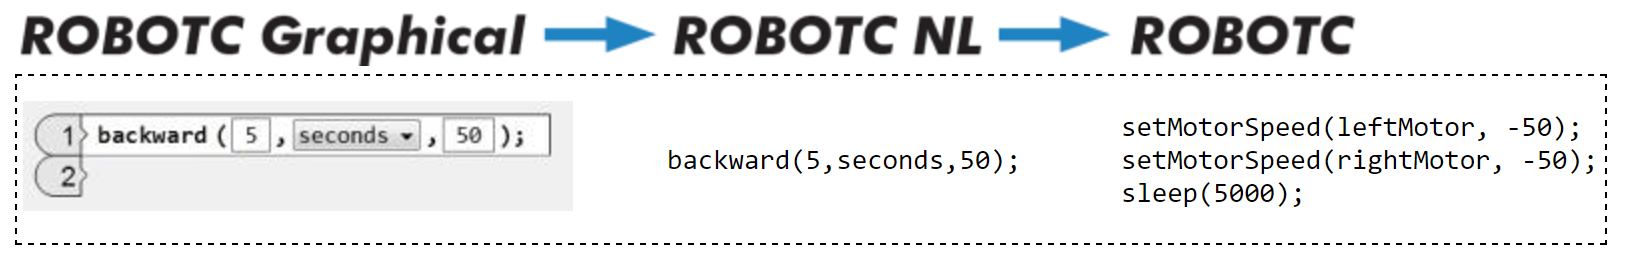
\includegraphics[width=330px]{images/robotc_language-variants.png}
	\caption[ROBOTC nabízí tyto varianty programování]{ROBOTC nabízí tyto varianty programování\protect\footnotemark} % CHECK: programování / programovacích jazyků
	\label{robotc_language-variants}
\end{figure}

\footnotetext{Zdroj: Oficiální nápověda v~programu ROBOTC -- záložka ROBOTC Language Progression} 

ROBOTC běží na standardním \lego{} systému podobně jako doplňky od~MathWorks nebo \NI{}.
Programy z~ROBOTC se na PC překládají do~byte-code aplikací a~následně se spouští na \brick{\it u} ve~virtuálním stroji. 
Tudíž zde může docházet k~podobným problémům, jako je popsáno v~kapitole~\ref{lego-soft-orig-problems}.

V~rámci vývojového programu pro toto prostředí je k~dispozici celá řada podpůrných nástrojů typu debugger, dataloger, vykreslování grafů nebo i~ovládání robota přes joystick.
Samotné prostředí je relativně propracované a~obsahuje mnoho funkcí. 
Aktuální verze by si zasloužila grafické přepracování tak, aby byla intuitivnější. 
Je trochu škoda, že není k~dispozici implementace jazyka ROBOTC v~C++ stylu, ale vzhledem k~dobré koncepci současného jazyka to asi není nutné. 

Jak bylo uvedeno v~úvodu, ROBOTC je komerční program, a~s~tím souvisí licenční politika. 
Ceny licencí s~platností na jeden rok jsou přibližně poloviční v~porovnání s~časově neomezenými verzemi.
Neomezená verze dle jednotlivých balíčků stojí: \$79, \$299, \$599~\cite{legoProgramingPlatform_ROBOTC-price}.  
V~porovnání s~produkty od MathWorks nebo \NI{} nejsou tyto sumy tak závratné a~když zvážíme cenu samotné stavebnice \legoEV{} (aktuálně 11 700 Kč~\cite{lego_eduxeEshop_CoreSet}, v~přepočtu přibližně~\$470), zdá se mi tato suma přijatelná.

I~tak může být cena za tento produkt pro mnohé uživatele, školy a~vzdělávací instituce rozhodující.
Zároveň kvůli uzavřenosti tohoto softwaru není možné jednoduše rozšiřovat funkcionalitu a~přidávat další vylepšení do programu. 
Vzhledem k~výše uvedeným důvodům jsem se rozhodl, že pro svou práci nebudu toto prostředí dále zvažovat.	


\section{EV3RT}
\label{lego-EV3RT}

Při hledání příčin problémů s~časováním na EV3~\cite{legoMindstormsEV3_ev3dev-issue_constant-loop-time} jsem narazil na zajímavý japonský projekt \evRT{}~\cite{legoProgramingPlatform_EV3RT-git-web}.
Jedná se o~port real-timového systému TOPPERS/HRP2 na \legoEV{}.
Projekt \evRT{} vznikl v~rámci výzkumu na Nagoya University v~Japonsku s~cílem odstranění problémů originálního \lego{} systému a~prostředí. 
Veškeré zdrojové kódy jsou volně k~dispozici na GitHubu~\cite{legoProgramingPlatform_EV3RT-github}. 

Historie projektu TOPPERS\footnote{TOPPERS = Toyohashi OPen Platform for Embedded Real-time Systems} sahá do roku 2003, kdy vznikl jako společný projekt průmyslu, univerzit a~vlády~\cite{legoProgramingPlatform_TOPPERS}. 
Cílem projektu bylo vytvoření kvalitního otevřeného real-time systému, využitelného v~průmyslu pro embedded zařízení. 
Zároveň měly být vytvořeny výukové kurzy a~materiály pro studenty.
V~Japonsku je tento systém využíván jak v~průmyslu, tak i~při výuce a~prakticky tvoří průmyslový standard pro embedded zařízení. 

TOPPERS je vyvíjen s~celou řadou real-time kernelů. Pro EV3 byl portován kernel s~označením HRP2\footnote{HRP2 = High Reliable system Profile version 2}.
Jedná se o~statický RTOS\footnote{RTOS = Real-Time Operating System} kernel s~podporou ochrany paměti, který splňuje vysokou spolehlivost a~bezpečnost aplikací~\cite{legoProgramingPlatform_EV3RT-paper}.
V~systému je možné vytvářet tasky (obdoba vláken v~Linuxu) s~různou prioritou. 
Jsou zde dostupné standardní prostředky pro komunikaci mezi tasky: semafory, mutexy, fronty.

\begin{figure}[h]
	\centering
	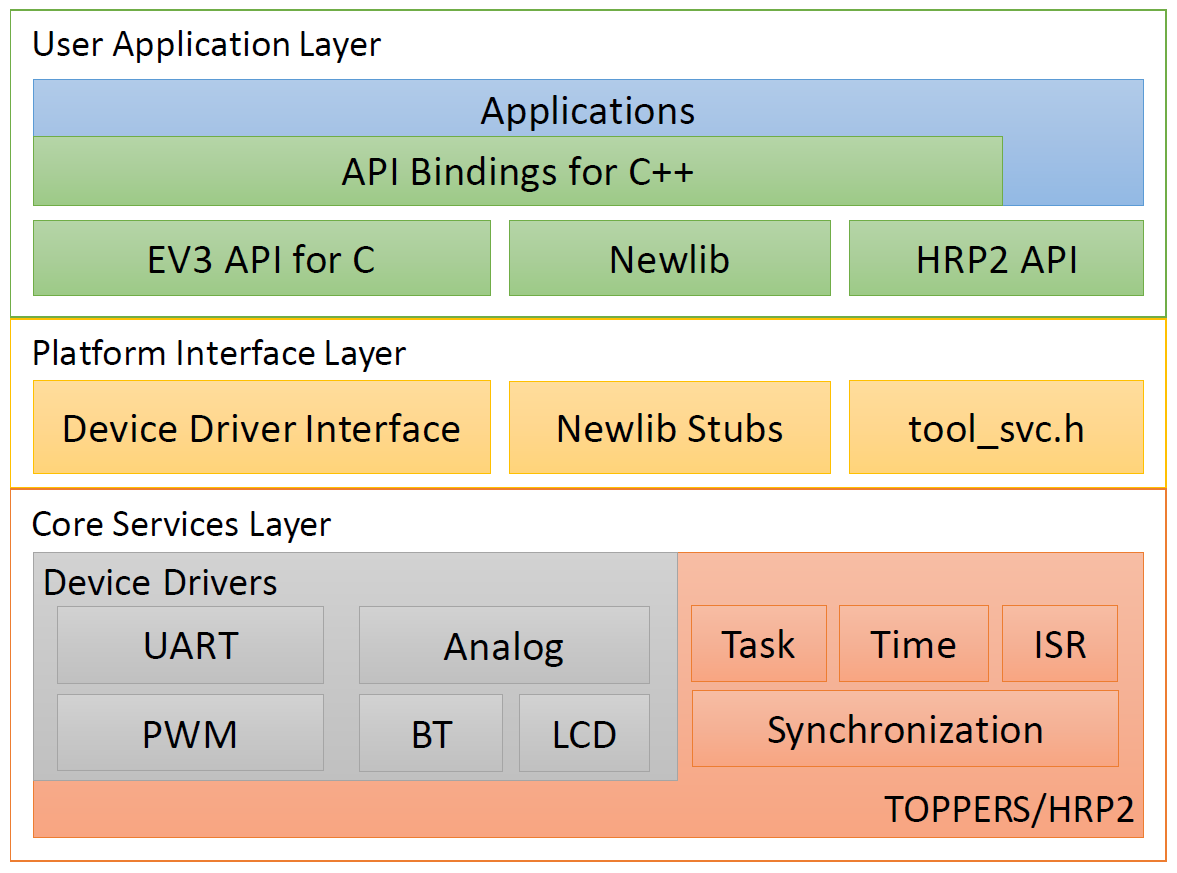
\includegraphics[width=330px]{images/ev3rt-architecture.png}
	\caption[Architektura systému EV3RT]{Architektura systému EV3RT\protect\footnotemark}
	\label{ev3rt-architecture}
\end{figure}

\footnotetext{Zdroj: článku A~Platform for LEGO Mindstorms EV3 Based on an RTOS with MMU Support~\cite{legoProgramingPlatform_EV3RT-paper}} 

V~rámci EV3RT jsou aktuálně podporovány všechny druhy senzorů a~motorů ze~stavebnice \legoEV{} a~fungují veškeré periferie na~\EVbrick{\it u} (displej, LED, tlačítka, Bluetooth a~reproduktor). 
Zatím není odzkoušená podpora pro NXT komponenty ani alternativní senzory a~motory. 

EV3RT poskytuje C~API pro přístup ke~všem funkcím na EV3. 
Jednoduše lze vyčíst hodnoty ze senzoru nebo roztočit motor.
Toto API není ale tak intuitivní, jak by mohlo být při použití C++.
K~dispozici je i~implementace dynamické alokace paměti a~lze tedy používat funkce \verb|malloc()| i~\verb|free()|.
Platforma nemá problém s~překladem standardní C++~knihovny (STL).
Uživatel tak může v~projektech využívat například \texttt{std::string}, \texttt{std::vector}, \texttt{std::queue}, \texttt{\dots}

Výkonnostně by na tom měl být systém EV3RT nejlépe ze všech platforem pro EV3, které byly zmíněny v~této kapitole. 
Hlavní příčinou je samotný RTOS, který má velmi nízkou režii na svůj chod a~umožňuje rychlý přístup k~hardwaru. % TODO: + rychlejší zpracování operaci a přepínání tasku
Oproti standardnímu \lego{} systému zde také neběží žádný virtuální stroj, který může výrazně degradovat výkon při některých operacích. 
Dle testů provedených tvůrci EV3RT je například provedení nastavení rychlosti ({\it motor\_set\_speed}) v~průměru až 100krát
 rychlejší než v~originálním systému~\cite{legoProgramingPlatform_EV3RT-paper}. \\
 
Shrnutí hlavních vlastností \evRT:

\begin{itemize}
	\item malá velikost systému (do 5 MB) i~uživatelských aplikací (do 1 MB)
	\item velmi rychlý start (do 5 sekund) a~prakticky okamžité vypnutí
	\item jednodušší úprava a~doprogramování vlastních funkcí do jádra systému
	\item snadné portování linuxových driverů
	\item podpora dynamické alokace paměti
	\item preemptivní multitasking s~velmi rychlým přepínáním kontextu (do 8 $\mu$s)
	\item multiplatformní vývoj aplikací pro EV3
\end{itemize}
 
Nevýhodou TOPPERS a~tedy i~EV3RT je, že se jedná primárně o~japonský projekt. 
Většina dokumentace k~TOPPERS je tak v~japonštině, což se týká i~velké části zdrojového kódu v~EV3RT. 
Části kódu, které byly převzaty z~oficiálního \lego{} systému nebo byly vytvářeny primárně pro EV3RT, jsou zdokumentovány v~angličtině. 

Například ale C~API obsahuje pouze japonskou dokumentaci.
Jedinou anglickou dokumentací k~funkcím dostupných v~TOPPERS/HRP2 je tak všeobecná RTOS specifikace $\mu$ITRON z~roku 2002~\cite{legoProgramingPlatform_TOPPERS-IRON}, kterou HRP2, a~tím pádem i~EV3RT, splňují. % splňují/implementují
Naštěstí překlad z~japonštiny do angličtiny zvládá Google Translate docela dobře, a~tak je možné tyto komplikace překonat.


Ačkoliv má EV3RT určité nevýhody popsané v~předchozím odstavci, rozhodl jsem se jej využít pro tvorbu programovacího prostředí pro \legoEV{}.
Tento systém jako jediný nabízí opravdovou real-timovost.
Netrpí degradací výkonu.
Zvládne velmi rychle nastartovat a~okamžitě se vypne. 
Nabízí relativně snadnou možnost zásahů do implementace (úpravu driverů pro EV3 -- úprava konstant PID~regulátoru, modifikace a~přidávání funkcí do uživatelského rozhraní, \dots). 

Pro EV3RT lze vyvíjet na libovolné POSIX-kompatibilní platformě obsahující GCC překladač pro procesory ARM. Vývoj je tedy možný jak na Linuxu a~Macu, tak i~na Windows s~použitím Cygwinu~\cite{legoProgramingPlatform_EV3RT-git-web_get-started}.


\section{Srovnání dostupných platforem}
\label{lego-soft-summary}

V~této kapitole shrnuji porovnání jednotlivých platforem mezi sebou. 
Vybral jsem několik bodů, které považuji za~důležité u~platformy určené pro programování stavebnice \lego{}. 
Zároveň by tyto body měly zohledňovat možnosti budoucího rozvoje daného prostředí a~snadné využití platformy ve~výuce. \\


Platformy budu posuzovat v~těchto bodech:

\begin{enumerate}
	\item dostupné zdarma
	\item open-source
	\item intuitivní programovací rozhraní pro neprogramátory
	\item nenáročnost na počáteční zprovoznění
	\item real-timovost
	\item nenáročné na hardware počítače
	\item možnost zásahů do vývojového prostředí
	\item podporované operační systémy
\end{enumerate}


\begin{center}
	\begin{tabular}{ | l | c | c | c | c | c | c | c | c |}
		\hline
		Prostředí:                  & 1      & 2      & 3      & 4      & 5      & 6      & 7     	& 8							\\ \hline
		Originální \lego{}          & \Has   & \NoHas & \Has   & \Has   & \NoHas & \NoHas & \NoHas 	& Windows, Mac	\\ \hline 
		\evThreeDev{}               & \Has   & \Has   & \NoHas & \NoHas & \NoHas & \Has   & \Has 	& Windows, Linux, Mac		\\ \hline 
		ROS 						& \Has   & \Has   & \NoHas & \NoHas & \NoHas & \NoHas & \Has 	& Linux						\\ \hline 
		MathWorks doplňky           & \NoHas & \NoHas & \NoHas & \Has   & \NoHas & \NoHas & \NoHas  & Windows, Linux, Mac		\\ \hline 
		\NI{} modul                 & \NoHas & \NoHas & \NoHas & \Has   & \NoHas & \NoHas & \NoHas  & Windows, Mac				\\ \hline
		ROBOTC		                & \NoHas & \NoHas & \Has   & \Has   & \NoHas & \Has   & \NoHas  & Windows					\\ \hline
		EV3RT			            & \Has   & \Has   & \NoHas & \NoHas & \Has   & \Has   & \Has   	& Windows, Linux, Mac		\\ \hline
	\end{tabular}
\end{center}

Z~výše uvedené tabulky i~hlubšího zkoumání jednotlivých prostředí v~rámci této kapitoly mi~jako nejvhodnější volba pro programování stavebnice \legoEV{} připadá prostředí EV3RT.
Má některé nedostatky, které u~jiných prostředí nejsou (složitější API, náročné na počáteční zprovoznění), ale právě tato problematická místa by mělo být možné díky otevřenému zdrojovému kódu odstranit.
Proto se již budu v~následujících kapitolách věnovat převážně tomuto systému.